\documentclass{iithesis}
\usepackage{polski}
\usepackage[utf8]{inputenc}

\usepackage{amsmath}
\usepackage{amsfonts}

\usepackage{graphicx}
\usepackage{dblfloatfix}
\usepackage{tikz}
\usetikzlibrary{shapes.geometric, arrows}
% \usetikzlibrary{decorations.pathmorphing}

\polishtitle    {Kompaktowe reprezentacje binarne i modele generatywne}
\englishtitle   {Compact binary representations and generative models}
\polishabstract {Niniejsza praca przedstawia możliwości zastosowania autoenkodera wariacyjnego
                (VAE) do znalezienia reprezentacji (w tym kompatkowej reprezentacji binarnej) dla chmur punktów 3D.
                W pracy opisano teoretyczne podstawy uczenia autoenkoderów wariacyjnych z regularyzacją
                zmiennej ukrytej rozkładem normalnym. Podano również przegląd metod wykorzystywanych do
                wymuszenia bardziej skomplikowanych rozkładów na zmiennej ukrytej (m.in. Gamma oraz Beta).
                Opisano również, w jaki sposób wykorzystać regularyzację rozkładem Beta do znalezienia kompatkowej
                reprezentacji binarnej dla chmur punktów 3D.
                Opisane modele zaimplementowano i przeprowadzono szereg eksperymentów sprawdzających ich zdolność
                rekonstrukcji oraz możliwości generatywne.}
\englishabstract{The following work demonstrates the possibility of using a variational autoencoder (VAE)
                for obtaining representations (including a compact binary one) for 3D point clouds.
                The paper includes theoretical baseline study of training variational autoencoders with
                a normally-distributed latent variable. Methods for regularization of the latent variable
                with a more complex distribution (such as Gamma or Beta) have also been presented.
                The work includes also a description of how to use a variational autoencoder with Beta
                regularization to obtain a compact binary representation for 3D point clouds.
                All described models have later been implemented and tested with a variety of experiments
                focusing on their reconstructive and generative capabilites.}
\advisor        {dr Rafał Nowak}
\author         {Jakub Zadrożny}
\date           {6 września 2019}

\begin{document}

\chapter{Wprowadzenie}
Modele generatywne, takie jak autoenkoder wariacyjny, stały się obecnie jednym z podstawowych narzędzi
do pracy z wielomami rodzajami danych od zdjęć twarzy do plików muzycznych.
Umożliwiają one znajdowanie efektywnych i interpretowalnych reprezentacji, które
pozwalają nie tylko na generowanie syntetycznych danych, ale rozwiązują również problemy takie
jak gładka inerpolacja pomiędzy dwoma obiektami, czy edycja poprzez ayrtmetykę na zmiennej ukrytej.

Obecnie jednak, dzięki popularyzacji urządzeń reprezentujących głębię obrazu,
takich jak LIDAR i kamera RGB-D, coraz większą rolę odgrywają chmury punktów 3D.
Wykorzystuje się je w wielu nowoczesnych, rewolucyjnych i kluczowych dla postępu technologiach,
m.in. pojazdach autonomicznych, robotyce oraz wirtualnej i rozszerzonej rzeczywistości.
Chmury punktów są dość skomplikowanymi danymi, które zajmują znacznie ilości miejsca i przetwarzane
w oryginalnej postaci nakładają spory narzut obliczeniowy. Dlatego istotnym zagadnieniem
jest znalezienie odpowiedniej reprezentacji dla takich danych. Taka reprezentacja
musi być kompaktowa, aby zmniejszyć narzut pamięciowy i obliczeniowy, a model powininen być generatywny,
żeby umożliwić tworzenie i edycję obiektów.

Chmury punktów 3D są aktywnym obszarem badań i na przestrzeni ostatnich lat powstało zarówno
wiele problemów (np. zbiory ShapeNet \cite{shapenet} i ModelNet40 \cite{modelnet}), jak i
rozwiązań (np. architektura PointNet \cite{pointnet} i metryka EMD \cite{emd}).
Niektóre z tych osiągnięć pozwalają tworzyć kolejne, bardziej zaawansowane modele,
m.in. opisany w tej pracy autoenkoder wariacyjny, który na podstawie znalezionej reprezentacji
potrafi rekonstruować i generować nowe chmury punktów.

Jednym ze znanych problemów VAE, jest trudność narzucenia na zmienną ukrytą niektórych mniej typowych rozkładów.
W dalszej częśc pracy opisano możliwe rozwiązania tego problemu, rozszerzające możliwości VAE,
dzięki którym da się regularyzować zmienną ukrytą np. rozkładem Gamma i Beta.
Podano również metodą, która pozwala wykorzystać VAE do znalezienia kompaktowej reprezentacji binarnej, która
pozwala zmniejszyć ilość przechowywanych i przetwarzanych danych -- kwestii kluczowej przy
stale rosnących rozmiarach i większej ilości danych.
Uzyskana reprezentacja zajmuje jedynie 128 bitów -- tyle, ile czterowymiarowa
reprezentacja ciągła -- jednak posiada znacznie większą zdolność rekonstrukcji, nie poświęcając
przy tym możliwości generatywnych.

Podsumuwując, praca składa się z czterech głównych części: (1) zawiera opis teoretycznych podstaw
autoenkodera wiaracyjnego, (2) podaje sposoby wymuszenia różnych rozkładów na zmiennej ukrytej,
(3) zawiera eksperymenty demonstrujące zdolności wytrenowanego modelu do rekonstrukcji,
generowania syntetycznych danych, interpolacji oraz edycji obiektów przez arytmetykę na zmiennej ukrytej
i (4) opsiuje sposób, w jaki można wykorzystać VAE z regularyzacją rozkładem Beta do otrzymania
kompaktowej (128 bitów) reprezentacji binarnej chmur punktów i potwierdza skuteczność tej
reprezentacji eksperymentami.

\chapter{Podstawy opracowania}

\section{Chmury punktów 3D}
Chmury punktów 3D reprezentują obiekty, kształty, powierzchnie w przestrzeni za pomocą zbioru
trójek liczb rzeczywistych: współrzędnych $x,y,z$ każdego z punktów.
Pojedynczą chmurę punktów reprezentuje zatem macierz wymiaru $N \times 3$ lub $3 \times N$,
gdzie $N$ -- liczba punktów. Ponieważ chmury reprezentowane są przez \textit{zbiór} punktów,
przyjmujemy, że dwie macierze różniące się tylko kolejnością wierszy (lub kolumn, zależnie od reprezentacji)
przedstawiają w rzeczywistości tę samą chmurę. Stwarza to dwa dodatkowe problemy: (1) cały model powinien
być niewrażliwy na permutacje wierszy macierzy wejściowej, (2) dekoder trzeba oceniać metryką niewrażliwą
na permutacje punktów.

\subsubsection{Architektura PointNet} \label{sec:related_pointnet}
Silnym narzędziem do pracy z chmurami punktów 3D jest architektura \textbf{PointNet} \cite{pointnet},
która umożliwa ekstrakcję cech (w pełni sparametryzowanych) z wejściowej chmury punktów.
Architektura ta posiada dwie podstawowe zalety istotne dla tej pracy: jest odporna na permutacje
punktów chmury wejściowej i przyjmuje jako wejście chmury w naturalnej postaci.
Inne metody rozwiązały problem permutacji przetwarzając chmury punktów na inne formaty (np. wykorzystujące voxele),
przez co rozmiar przetwarzanych danych i czas obliczeń wzrasta. PointNet osiąga ten sam cel, zachowując
względną prostotę modelu, co z uwagi na ograniczone zasoby obliczniowe jest kluczowe.

\subsubsection{Metryki}
Powszechnie stosuje się dwie metryki dla chmur punktów 3D \cite{metrics}. Załóżmy, że mamy dwa zbiorzy
$S_1 \in \mathbb{R}^3$ i $S_2 \in \mathbb{R}^3$.

\textit{Chamfer} pseudo-distance (\textbf{CD}), która dla każdego punktu z $S_1$ oblicza
odległość od najbliższego punktu w $S_2$ i odwrotnie. Dana jest wzorem
\begin{equation} \label{eq:chamfer_intro}
CD(S_1, S_2) = \sum_{x \in S_1} \min_{y \in S_2} ||x-y||_2^2 + \sum_{y \in S_2} \min_{x \in S_1} ||x-y||_2^2
\end{equation}

Earth-mover distance (\textbf{EMD}) \cite{emd}, która znajduje permutację punktów wyjściowego zbioru,
dla której suma odległości punkt po punkcie jest najmniejsza. Dana jest wzorem
\begin{equation}
EMD(S_1, S_2) = \min_{\Phi:S_1 \rightarrow S_2} \sum_{x \in S_1} ||x-\Phi(X)||_2^2
\end{equation}
gdzie $\Phi$ jest bijekcją.

Jak zaznaczają autorzy \cite{pc_representations}, użycie metryki EMD pozwala uzyskać lepsze rezultaty
w rekonstrukcji obiektów, jednak jej wyliczanie jest znacznie bardziej kosztowen niż CD, dlatego
w tej pracy skupiono się na metryce CD.

\section{Autoenkodery}
Podstawowym modelem opisywanem w tej pracy jest autoenkoder \cite{autoencoders}. Autoenkoder to model
złożony z dwóch sieci neuronowych: \textbf{enkodera} i \textbf{dekodera}. Sieci trenuje
się wspólnie, w taki sposób, aby na podstawie wyniku zwróconego przez enkoder, dekoder był w stanie
zrekonstruować oryginalne dane (wejście do enkodera). Autoenkodery stają się praktyczne, gdy
nałoży się ograniczenie na dane przekazywane pomiędzy enkoderem i dekoderem
(nazywane zmienną ukrytą lub \textit{reprezentacją}),
np. ograniczy się mocno ich wymiar. Schemat działania enkodera przedstawia rys. \ref{fig:ae_basics}.

\begin{figure}[b]
    \center{
        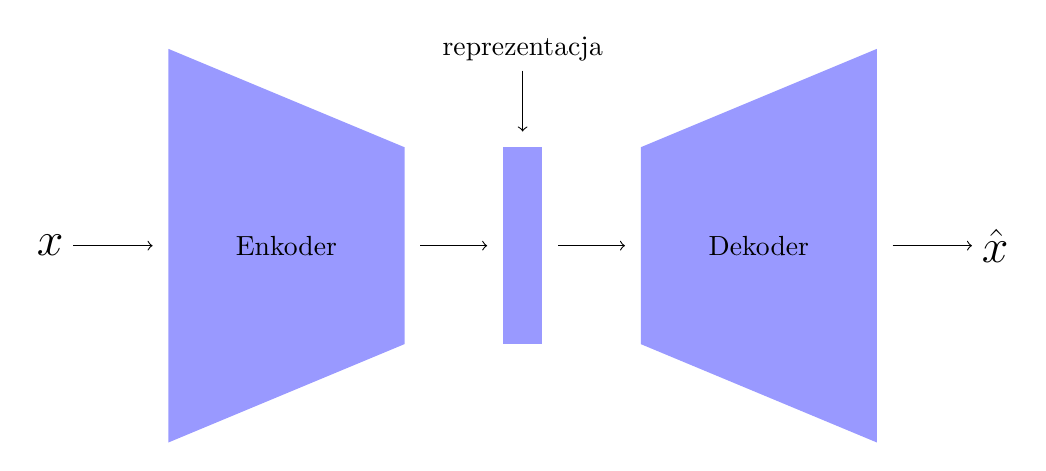
\begin{tikzpicture}
            \fill[blue!40!white] (-4.5,2.5) -- (-4.5,-2.5) -- (-1.5,-1.25) -- (-1.5,1.25) -- cycle;
            \node[inner sep=0pt] at (-3,0) {Enkoder};
            \fill[blue!40!white] (1.5,1.25) -- (1.5,-1.25) -- (4.5,-2.5) -- (4.5,2.5) -- cycle;
            \node[inner sep=0pt] at (3,0) {Dekoder};
            \fill[blue!40!white] (-0.25,1.25) -- (-0.25,-1.25) -- (0.25,-1.25) -- (0.25,1.25) -- cycle;
            \draw[->] (-1.3,0) -- (-0.45,0);
            \draw[->] (0.45,0) -- (1.3,0);
            \node[] at (-6,0) (input) {\LARGE $x$};
            \draw[->] (input) -- (-4.7,0);
            \node[] at (6,0) (output) {\LARGE $\hat{x}$};
            \draw[->] (4.7,0) -- (output);
            \node[] at (0,2.5) (repr) {reprezentacja};
            \draw[->] (repr) -- (0,1.45);
        \end{tikzpicture}
    }
    \caption{\label{fig:ae_basics} Schemat działania autoenkodera. Celem jest uzyskanie $\hat{x}$
    jak najbliższego $x$.}
\end{figure}

\section{Modele generatywne}
Klasycznym wynikiem, który spopularyzował modele generatywne, jest autoenkoder wariacyjny
(\textbf{VAE}) \cite{vae}. Jego najważniejszą zaletą jest probabilistyczny charakter,
dzięki czemu możemy żądać, aby zmienna ukryta (\textit{latent}) była zradnomizowana i pochodziła
z pewnego zadanego rozkładu prawdopodobieństwa (z pewnymi ograniczeniami).
Dzięki randomizacji zmiennych ukrytych uzyskujemy zagęszczenie przestrzeni reprezentacji,
przez co niemal każdy punkt może zostać zdekodowany na realistyczne dane.
Umożliwia to realizowanie zadań takich jak generowanie syntetycznych,
realistycznych danych lub gładkie interpolacje znaczeniowe obiektów.

\section{Estymacja gradientu wartości randomizowanych}
Do wytrenowania autoenkodera wariacyjnego używa się najczęściej wariantu metody SGD, która
wymaga wyliczania pochodnych funkcji kosztu po kolejnych parametrach modelu, co z kolei
wymaga wyliczania pochodnych wartości pojawiających się we wszystkich warstwach po parametrach
wartstw poprzednich (propagacja wstecz).
Do wyliczenia funkcji kosztu w VAE używa się szacowania Monte Carlo, które opiera się na
próbkowaniu zmiennej losowej. Oznacza to, że do wytrenowania autoenkodera wariacyjnego
niezbędne jest obliczanie pochodnych wylosowanej zmiennej po parametrach rozkładu.
W tym celu stosouje się dwie postawowe metody.

Estymator \textbf{score function} opisany m.in. w \cite{score_fn} oferuje stosunkowo
proste przybliżenie gradientu funkcji kosztu i można go stosować do szerokiej gamy rozkładów,
jednak charakteryzuje się dużą wariancją oszacowania, co komplikuje proces trenowania.

Drugim podejściem jest \textbf{pathwise gradients}, czyli tzw. trik repearametryzacyjny
opsisywany m.in. w \cite{vae}. Metoda ta opiera się na przedstawieniu zmiennej $z$ pochodzącej
z rozkładu $q(z;\theta)$ sparametryzowanego przez $\theta$ jako $z=\mathcal{T}(\epsilon;\theta)$,
gdzie $\epsilon$ pochodzi z pewnego rokładu $q_0$ niezależnego od $\theta$, a
$\mathcal{T}$ jest obliczalnym i różniczkowalnym po $\theta$ przekształceniem.
Trik repearametryzacyjny jest łatwy do zastosowania dla części stosowanych rozkładów
(szczególnie dla tych z rodziny kształtu i skali), jednak z uwagi na brak prostego przekształcenia
$\mathcal{T}$ nie da się go wprost zastosować do niektórych istotnych rozkładów, np. Gamma i Beta.

Rozszerzenie tej metody na kolejne rodziny rozkładów zostało zaproponowane w \cite{pathwise_gradients}.
Autorzy wprowadzają metodę, która pozwala w efektywny sposób szacować gradienty funkcji kosztu,
nawet gdy zmienne pośrednie pochodzą ze skomplikowanych rozkładów jak Gamma i Beta.

% \section{Klasteryzacja}

\chapter{Metody}
\section{Autoenkoder wariacyjny z rozkładem normalnym}
\label{sec:vae_normal}
Autoenkodery wariacyjne są dobrze znane i zbadane pod kątem niektórych zagadnień,
np. analizy obrazów. Jednak zastosowanie ich do chmur punktów 3D wymaga opracowania
dokładniejszej metody.

Dalej zakładamy, że dysponujemy zbiorem danych
$$
\mathcal{X} = \{x_i \in \mathbb{R}^{d}\}_{i \in I}
$$
dla pewnego $d$ -- wymiaru. Ponadto zakładamy, że dane te są obserwacjami
zmiennej losowej o rozkładzie następującej postaci
\begin{equation}
f(z, x; \theta) = f(z)f(x|z; \theta)
\label{eq:generative_process_factorization}
\end{equation}
gdzie $z \in \mathbb{R}^k$ dla pewnego $k$ (wymiar przestrzeni reprezentacji) -- zmienna pośrednia (\textit{latent}), $x \in \mathbb{R}^d$ -- zmienna obserwowana,
a $\theta$ -- parametr rozkładu. Dodatkowo niech
\begin{equation}
\begin{split}
z &\sim \mathcal{N}(0, I_k) \\
x|z &\sim \mathcal{N}(\mu_x(z; \theta), \mu_\sigma(z;\theta)I_d)
\end{split}
\label{eq:generative_process_distribs}
\end{equation}
gdzie $\mu_x,\,\mu_{\sigma}$ są skomplikowanymi obliczeniami
wykonywanymi przez sieć neuronową sparametryzowaną przez $\theta$.

\subsection{ELBO} \label{sec:elbo}
Naszym celem jest odtworzenie parametrów rozkładu generującego $\theta$
oraz rozkładu $f(z|x; \theta)$, który nazywamy \textit{reprezentacją} danych
generowanych przez proces opsiany w
(\ref{eq:generative_process_factorization}) i (\ref{eq:generative_process_distribs}).

Niestety z powodu zastosowania skomplikowanych, nieliniowych
transformacji dokładne odtworzenie rozkładu $f(z|x; \theta)$ jest niemożliwe.
W tym celu wprowadzamy pewne przybliżenie tego rozkładu -- nazwijmy je
$g(z|x; \phi)$.

Niech $g(z|x; \theta)$ będzie gęstością
rozkładu normalnego ze średnią $\rho_x(x; \phi)$ i wariancją $\rho_{\sigma}(x; \phi)$,
gdzie $\rho_x,\,\rho_{\sigma}$ są reprezentowane przez sieci neuronowe
parametryzowane przez $\phi$. Wtedy
\begin{equation}
\begin{split}
KL(g(z|x;\phi) || f(z|x;\theta)) &= \mathbb{E}_{z\sim g(z|x;\phi)}\left[
-\log\frac{f(z|x;\theta)}{g(z|x;\phi)}\right]= \\
&=\mathbb{E}_{z\sim g(z|x;\phi)}\left[-\log\frac{f(z|x;\theta)f(x;\theta)}{g(z|x;\phi)f(x;\theta)}\right]= \\
&=\mathbb{E}_{z\sim g(z|x;\phi)}\left[-\log\frac{f(z|x;\theta)f(x;\theta)}{g(z|x;\phi)}+\log f(x;\theta)\right] \\
&=\mathbb{E}_{z\sim g(z|x;\phi)}\left[-\log\frac{f(z,x;\theta)}{g(z|x;\phi)}\right] +\log f(x;\theta)
\end{split}
\end{equation}
gdzie $KL(\cdotp || \cdotp)$ jest odległością Kullbacka-Leiblera \cite{kl-cost}.
Zatem
\begin{equation}
\log f(x;\theta) = KL(g(z|x;\phi) || f(z|x;\theta)) + \mathbb{E}_{z\sim g(z|x;\phi)}\left[\log\frac{f(z,x;\theta)}{g(z|x;\phi)}\right]
\end{equation}
Ponieważ $KL(\cdotp || \cdotp) \geq 0$, więc
\begin{equation}
\begin{split}
\log f(x;\theta)  &\geq \mathbb{E}_{z\sim g(z|x;\phi)}\left[\log\frac{f(z,x;\theta)}{g(z|x;\phi)}\right] = \\
&= \mathbb{E}_{z\sim g(z|x;\phi)}\left[\log\frac{f(x|z;\theta)f(z)}{g(z|x;\phi)}\right] = \\
&=\mathbb{E}_{z\sim g(z|x;\phi)}\left[\log f(x|z;\theta)\right] - \mathbb{E}_{z\sim g(z|x;\phi)}\left[-\log\frac{f(z)}{g(z|x;\phi)}\right] =\\
&=\mathbb{E}_{z\sim g(z|x;\phi)}\left[\log f(x|z;\theta)\right] - KL(g(z|x;\phi) || f(z))
\end{split}
\label{eq:elbo}
\end{equation}
Zatem dla dowolnego rozkładu aproksymującego $g(z|x;\phi)$ otrzymujemy dolne
ograniczenie na prawdopodobieństwo wygenerowania zaobserwowanych danych.
Dlatego część wzoru po prawej stronie od ostatniej równości
nazywamy \textbf{ELBO} (\textit{evidence lower bound}). Możemy zauważyć, że ostateczna
postać wzoru (\ref{eq:elbo}) składa się z dwóch części naturalnie odpowiadającymi dwóm
celom, które chcemy zoptymalizować: pierwszy składnik odpowiada
jakości rekonstrukcji obserwacji ze zmiennej ukrytej $z$
(dlatego nazywany jest kosztem rekonstrukcji),
natomiast drugi to odległość KL rozkładu aproksymującego
$f(z|x;\theta)$ od naszego założenia na jego temat.

\subsection{Zadanie optymalizacyjne} \label{sec:optim_task}
Chcemy znaleźć układ parametrów $<\theta,\,\phi>$, który daje najlepszą
gwarancję na prawdopodobieństwo wygenerowania zaobserwowanych danych (ELBO).
W tym celu posłużymy się lekko zmodyfikowanym algorytmem SGD.
Naszym zadaniem jest znalezienie
\begin{equation}
\label{eq:loss_f}
\begin{split}
\max_{\theta,\,\phi} \hat{\mathcal{L}}(\mathcal{X}, \theta, \phi) &= \sum_{i \in I}\mathcal{L}(x_i, \theta, \phi) = \\
&=\sum_{i \in I} \left( \mathbb{E}_{z\sim g(z|x_i;\phi)}\left[\log f(x_i|z;\theta)\right] - KL(g(z|x_i;\phi) || f(z)) \right)
\end{split}
\end{equation}
Ponieważ bardziej naturalnym zadaniem jest minimalizowanie funkcji kosztu,
to rozwiążemy równoważne zadanie znalezienia
\begin{equation}
\min_{\theta,\,\phi} -\hat{\mathcal{L}}(\mathcal{X}, \theta, \phi)
\end{equation}

Żeby posłużyć się algorytmem SGD musimy umieć wyliczać i różniczkować
oba składniki funckji $\mathcal{L}$.

\subsection{Koszt KL}
Odległość KL dwóch rozkładów normalnych o następujących parametrach
\begin{equation*}
\begin{split}
\mathcal{N}_0 \sim \mathcal{N}(\mu_0, \Sigma_0) \\
\mathcal{N}_1 \sim \mathcal{N}(\mu_1, \Sigma_1)
\end{split}
\end{equation*}
dla pewncyh $\mu_0,\,\mu_1 \in \mathbb{R}^k,\ \Sigma_0, \Sigma_1 \in \mathbb{R}^{k \times k}$, wynosi
\begin{equation*}
KL(\mathcal{N}_0||\mathcal{N}_1) = \frac{1}{2} \left(\text{tr}(\Sigma_1^{-1}\Sigma_0)
+ (\mu_1-\mu_0)^T \Sigma_1^{-1} (\mu_1-\mu_0) -k + \log\frac{\det\Sigma_1}{\det\Sigma_0} \right)
\end{equation*}
Ponieważ zakładamy, że $f(z)$ jest rozkładem $z \sim \mathcal{N}(0, I_k)$, więc
\begin{equation}
KL(g(z|x;\phi) || f(z)) = \frac{1}{2}\sum_{i=1}^k
\left( \rho_x(x;\phi)_i^2 + \rho_\sigma(x;\phi)_i^2 - \log(\rho_\sigma(x;\phi)_i^2)-1 \right)
\label{eq:kl_loss}
\end{equation}
Wzór (\ref{eq:kl_loss}) można wyliczać i różniczkować analitycznie.

\subsection{Koszt rekonstrukcji} \label{sec:rec_loss_normal}
Drugiego składnika funckji $\mathcal{L}$, czyli kosztu rekonstrukcji,
nie da się wyznaczyć analitycznie. Aby objeść ten problem, możemy metodą Monte Carlo
oszacować wartość oczekiwaną przez średnią
$$
\mathbb{E}_{z\sim g(z|x;\phi)}\left[\log f(x_i|z;\theta)\right] \sim
\frac{1}{m} \sum_{i=1}^m -\log f(x|z_i;\theta)
$$
gdzie $z_i \sim g(z|x;\phi)$. Taką wartość potrafimy już wyliczyć, ale nie
potrafimy propagować gradientu do parametrów $\phi$ przez
zaobserwowane wartości $z_i$.

Wprowadzimy repearametryzację zmiennych $z_i$ -- możemy zauważyć, że zmienna
$z_i=\rho_x(x;\phi)+\epsilon_i\rho_\sigma(x;\phi)$
gdzie $\epsilon_i \sim \mathcal{N}(0, I_k)$
ma rozkład $g(z|x;\phi)$ a ponadto możemy propagować gradient do parametrów $\phi$.
Otrzymaliśmy zatem następujące przybliżenie na $\mathcal{L}$
$$
\mathbb{E}_{z\sim g(z|x;\phi)}\left[\log f(x_i|z;\theta)\right] \sim
\frac{1}{m} \sum_{i=1}^m -\log f(x|z_i=\rho_x(x;\phi)+\epsilon_i\rho_\sigma(x;\phi);\theta)
$$
gdzie $\epsilon_i \sim \mathcal{N}(0, I_k)$

Ponieważ $x|z \sim \mathcal{N}(\mu_x(z; \theta), \mu_\sigma(z;\theta)I_d)$, więc
$$
-\log f(x|z;\theta)=\sum_{i=1}^d \left( \frac{1}{2}\log(2\pi) +\log(\mu_\sigma(z;\theta)_i)
+\frac{(x-\mu_x(z;\theta)_i)^2}{2\mu_\sigma(z;\theta)_i^2} \right)
$$
jednak metryka ta niezbyt dobrze nadaje się do chmur punktów, ponieważ np.
chcielibyśmy uznawać permutację punktów oryginalnej chmury za dobrą rekonstrukcję.
Dlatego zamiast wyliczać \textit{stricte} $\log f(x|z;\theta)$ skorzystamy ze zmodyfikowanego
\textit{Chamfer distance} danego wzorem
\begin{equation}
CD(\mathcal{X}_1,\mathcal{X}_2) = \sum_{x \in \mathcal{X}_1} \min_{y \in \mathcal{X}_2} ||x-y||_2^2
+ \sum_{x \in \mathcal{X}_2} \min_{y \in \mathcal{X}_1} ||x-y||_2^2
\label{eq:chamfer_distance}
\end{equation}
gdzie $\mathcal{X}_1,\,\mathcal{X}_2$ są zbiorami punktów wielowymiarowych.
Ściślej mówiąc, możemy potraktować $\mu_x(z;\theta) \in \mathbb{R}^{3 \cdotp m}$ jako chmurę
$m$ punktów trójwymiarowych, oznaczmy ją $\hat{y}$. Ponadto dla $y \in \hat{y}$ niech
$\sigma(y)$ oznacza 3-elementowy wektor wariancji $\mu_\sigma(z;\theta)$ utworzony ze
składowych odpowiadających $y$. Za koszt rekonstrukcji przyjmiemy
\begin{equation}
\begin{split}
\mathcal{L}_{rec}(\hat{x}|z,\theta,\phi) &= \sum_{x \in \hat{x}} \min_{y \in \hat{y}}
\left( -\log p_{y,\sigma(y)}(x) \right) +\\
&+ \sum_{y \in \hat{y}} \min_{x \in \hat{x}} \left( -\log p_{x,\sigma(y)}(y) \right)
% \sum_{i=1}^3 \log(\mu_\sigma(z;\theta)_{y,i})+\frac{(x_i-y_i)^2}{2\mu_\sigma(z;\theta)_{y,i}^2} + \\
% &+ \sum_{x \in \mu_x(z|\theta) \min_{y \in \hat{x}}
% \sum_{i=1}^3 \log(\mu_\sigma(z;\theta)_{y,i})+\frac{(x_i-y_i)^2}{2\mu_\sigma(z;\theta)_{y,i}^2}
\end{split}
\end{equation}
gdzie $p_{v,s}(x)$ jest gęstością rozkładu normalnego o średniej $v$ i macierzy kowariancji
$sI$ w punkcie $x$.

Po usunięcu stałych wyrazów można to zapisać jako
\begin{equation} \label{eq:rec_loss}
\begin{split}
\mathcal{L}_{rec}(\hat{x}|z,\theta,\phi) &= \sum_{x \in \hat{x}} \min_{y \in \hat{y}} \sum_{i=1}^3
\left( \log(\sigma(y)_i) + \frac{(x_i-y_i)^2}{2\sigma(y)_i^2} \right) +\\
&+ \sum_{y \in \hat{y}} \min_{x \in \hat{x}} \sum_{i=1}^3
\left( \log(\sigma(y)_i) + \frac{(x_i-y_i)^2}{2\sigma(y)_i^2} \right)
\end{split}
\end{equation}
W obecnej wersji modelu dla uproszczenia przyjęto, że $\mu_\sigma(z;\theta) = \alpha$
dla wszystkich $z$ i niezależnie od parametrów $\theta$ (tzn. przyjęto stałą wariancję dla
danych wyjściowych). Wtedy wzór (\ref{eq:rec_loss}) upraszcza się do
\begin{equation} \label{eq:final_rec_loss}
\begin{split}
\mathcal{L}_{rec}(\hat{x}|z,\theta,\phi) &= \frac{1}{2\alpha^2} \left(
\sum_{x \in \hat{x}} \min_{y \in \hat{y}} ||x-y||_2^2 +
\sum_{y \in \hat{y}} \min_{x \in \hat{x}} ||x-y||_2^2 \right) = \\
&= \frac{1}{2\alpha^2} CD(\hat{x}, \hat{y})
\end{split}
\end{equation}

\section{Autoenkoder wariacyjny z rozkładem Beta} \label{sec:vae_beta}
Podobnie jak w sekcji \ref{sec:vae_normal} załóżmy, że posiadane przez nas dane
są obserwacjami pewnej zmiennej losowej. Tym razem postawmy jednak założenie, że
$z$ jest $k$-wymiarową zmienną, której składowe $z_i$ są niezależne oraz
$$
z_i \sim \text{Beta}(0.01, 0.01)
$$
dla $1 \leq i \leq k$, podczas gdy rozkład $x|z$ jest taki jak w (\ref{eq:generative_process_distribs}).

Rozkład $\text{Beta}(0.01, 0.01)$ (rys. \ref{fig:beta_distrib}) jest bardzo silnie
skupiony przy brzegach nośnika, t.j. 0 i 1. Przez regularyzowanie autoenkodera takim rozkładem
chcemy, aby otrzymywane zmienne pośrednie były również bardzo blisko 0 i 1, dzięki czemu
po ich zaokrągleniu i przekazaniu do dekodera błąd rekonstrukcji nie wzrośnie znacząco.

\begin{figure}
    \center{\includegraphics[width=0.7\textwidth]{images/beta_distrib.png}}
    \caption{\label{fig:beta_distrib} Gęstość rozkładu $\text{Beta}(0.01, 0.01)$.
    Istotne dla modelu jest silne skupienie gęstości przy brzegach nośnika.}
\end{figure}

Analogicznie do sekcji \ref{sec:elbo} wprowadzamy przybliżenie $g(z|x;\phi)$
dla nieznanego rozkładu $f(z|x;\theta)$. W tym przypadku niech $g(z|x;\phi)$
będzie iloczynem funkcji $g_i(z|x;\phi)$, z których każda jest gęstością rozkładu
$\text{Beta}(\alpha_i, \beta_i)$, gdzie
\begin{equation*}
\begin{aligned}[t]
\begin{bmatrix}
\alpha_1 \\
\vdots \\
\alpha_k
\end{bmatrix}
= \rho_\alpha(x;\phi)
\end{aligned}
\qquad \qquad
\begin{aligned}[t]
\begin{bmatrix}
\beta_1 \\
\vdots \\
\beta_k
\end{bmatrix}
= \rho_\beta(x;\phi)
\end{aligned}
\end{equation*}
gdzie $\rho_\alpha,\ \rho_\beta$ są ponownie reprezentowane przez sieci neuronowe
parametryzowane przez $\phi$. Innymi słowy, $g(z|x;\phi)$ jest rozkładem łącznym
niezależnych zmiennych o rozkładach Beta z różnymi parametrami.

Przy tych założeniach wszystkie obliczenia wykonywane w sekcji \ref{sec:elbo}
są dalej poprawne i możemy wykorzystać ELBO (wzór (\ref{eq:elbo})) do
określenia analogicznego zadania optymalizacyjnego (jak w sekcji \ref{sec:optim_task})
i zadania funkcji kosztu wzorem (\ref{eq:loss_f}).

\subsection{Koszt KL}
Odległość KL dwóch jednowymiarowych rozkładów Beta o następujących parametrach
\begin{equation*}
\begin{split}
\beta_0 \sim \text{Beta}(\alpha_0, \beta_0) \\
\beta_1 \sim \text{Beta}(\alpha_1, \beta_1)
\end{split}
\end{equation*}
dla pewnych $\alpha_0,\alpha_1,\beta_0,\beta_1 \in \mathbb{R}_{+}$ wynosi
\begin{equation} \label{eq:univariate_beta_kl}
\begin{split}
KL(\beta_0 || \beta_1) &= \log \left( \frac{\text{B}(\alpha_1,\beta_1)}{\text{B}(\alpha_0,\beta_0)} \right)
+ (\alpha_0-\alpha_1)\psi(\alpha_0) +\\
&+ (\beta_0-\beta_1)\psi(\beta_0) + (\alpha_1-\alpha_0+\beta_1-\beta_0)\psi(\alpha_0+\beta_0)
\end{split}
\end{equation}
gdzie $\text{B}(x,y)=\frac{\Gamma(x)\Gamma(y)}{\Gamma(x+y)}$ to funkcja beta,
a $\psi(x)=\frac{\Gamma'(x)}{\Gamma(x)}$ to funkcja digamma.
Procedury wyliczające obie funkcje (beta i digamma) efektywnie i stabilnie numerycznie
są szeroko dostępne w bibliotekach (m.in. używanej w tym projekcie bibliotece PyTorch).

Ponadto odległość KL jest addytywna dla zmiennych niezależnych, zatem
\begin{equation*}
KL(g(z|x;\phi) || f(z)) = \sum_{i=1}^k
KL(\text{Beta}(\rho_\alpha(x;\phi)_i,\rho_\beta(x;\phi)_i) || \text{Beta}(0.01,0.01)
\end{equation*}
Składniki tej sumy możemy wyliczać na podstawie równania (\ref{eq:univariate_beta_kl}).

\subsection{Koszt rekonstrukcji} \label{sec:rec_loss_beta}
W sekcji \ref{sec:rec_loss_normal} wprowadzamy szacowanie kosztu rekonstrukcji metodą Monte Carlo
$$
\mathbb{E}_{z\sim g(z|x;\phi)}\left[\log f(x_i|z;\theta)\right] \sim
\frac{1}{m} \sum_{i=1}^m -\log f(x|z_i;\theta)
$$
gdzie $z_i$ są próbkami z rozkładu $g(z|x;\phi)$. Aby wytrenować enkoder potrzebujemy wyliczyć
$$
\nabla_\phi f(x|z_i;\theta)
$$
jednak nie możemy tego zrobić wprost, gdy zmienne $z_i$ zależą od parametrów $\phi$ poprzez
operację próbkowania. Byłoby to możliwe, gdybyśmy przedstawili zmienne $z_i$ jako
obliczalną i różniczkowalną po parametrach $\phi$ transformację
zmiennej wylosowanej z pewnego rozkładu standardowego, niezależnego od parametrów
(zachowując odpowiedni rozkład $z_i$). Podejścia tego użyliśmy już w sekcji \ref{sec:rec_loss_normal}
reparametryzując $z \sim \mathcal{N}(\mu, \sigma)$ jako $z=\mu + \sigma \epsilon$,
gdzie $\epsilon \sim \mathcal{N}(0, 1)$.

Podobny trik można zastosować do innych rozkładów z rodziny położenia i skali, niestety
jednak nie działa on z rozkładami takimi jak Gamma i Beta, którego używamy w tym modelu.

Bardziej ogólnym kandydatem na taką transformację jest $z = F^{-1}(u;\phi)$,
gdzie $F^{-1}$ to odwrtoność dystrubuanty rozkładu $g(z|x;\phi)$, a $u \sim \mathcal{U}(0, 1)$.
Dla rozładów Gamma i Beta to podejście również nie jest wystarczające, gdyż
ich odwrotna dystrubuanta nie daje się przedstawić zwartym wzorem.

Można rozważać dwa rozwiązania powyższego problemu. Pierwsze to przybliżenie
odwrotności dystrubuanty funkcją obliczalną i różniczkowalną.
Drugie podejście korzysta z faktu, że
$$
u = F(z;\phi)
$$
Obie strony równości różniczkujemy po $\phi$ i korzystamy z tego, że $u$ nie zależy od parametrów $\phi$.
Otrzymujemy
$$
0 = \frac{dz}{d\phi}g(z|x;\phi)+\frac{\partial F(z;\phi)}{g(z|x;\phi)}
$$
co daje
\begin{equation} \label{eq:implicit_gradient}
\frac{dz}{d\phi} = -\frac{\frac{\partial F(z;\phi}{g(z|x;\phi)}}{g(z|x;\phi)}
\end{equation}
Równanie \ref{eq:implicit_gradient} pozwala wyliczać pochodne wylosowanej zmiennej $z$
po parametrach rozkładu, jeżeli mamy możliwość wyliczania lub przybliżania pochodnych
dystrubuanty $F$.

Dla rozkładów Gamma i Beta oba rozwiązania wymagają przybliżania funkcji
jej różniczkowalną wersją. Drugie podejście posiada jednak tę zaletę,
że nie wpływa na proces losowania zmiennych $z_i$, dzięki czemu możemy do tego użyć
dokładniejszej procedury i zapewnić odpowiedni rozkład $z_i$. Pierwsze podejście
tymczasem wprowadza przybliżenie już na etapie wyciągania próbki, co oznacza, że zmienne
$z_i$ mają rozkład $g(z|x;\phi)$ tylko w przybliżeniu.

% Dodać może szczegóły o przybliżeniu?
Najprostszym, ale niezbyt dokładnym, sposobem przybliżenia pochodnej dystrubuanty
rozkładu Gamma lub Beta jest policzenie ilorazów różnicowych.
Wymaga to jedynie porcedur wyliczających gęstość tych rozkładów,
które są szeroko dostępne w bibliotekach.
Autorzy \cite{pathwise_gradients} proponują znacznie dokładniejsze (i bardziej skomplikowane)
przybliżenie, które również zostało zaimplementowane w bibliotece PyTorch \cite{pytorch}.

\noindent \textit{Uwaga.} W powyższym opisie skupiliśmy się na rozkładach Beta oraz Gamma,
mimo że w dalszej części wykorzystujemy jedynie rozkład Beta. Rozkład Gamma pojawia się dlatego,
że gdybyśmy rozwiązali dla niego rozważany problem, to korzystając z faktu, że $Y = \frac{X_1}{X_1+X_2}$
ma rozkład $\text{Beta}(\alpha,\beta)$, gdy $X_1 \sim \text{Gamma}(\alpha,\theta),\ X_2 \sim \text{Gamma}(\beta,\theta)$,
otrzymujemy rozwiązanie dla rozkładu Beta (ta transformacja jest różniczkowalna).
Autorzy \cite{pathwise_gradients} zaznaczają jednak, że ten sposób wprowadza do metody dodatkową wariancję
i proponują lepsze rozwiązanie. Mimo tego w implementacji użyto powyższego triku.

Mając do dyspozycji wylosowane zmienne $z_i$, dla których możemy propagować gradient
wstecz, używamy estymatora Monte Carlo i kosztu rekonstrukcji jak w równaniu (\ref{eq:final_rec_loss}).

% \section{Model \textit{M2} Kingmy}
% \section{Autoenkoder wariacyjny z mieszanką gaussowską}

\chapter{Implementacja i architektura modeli}
Metody opsiane w sekcjach \ref{sec:vae_normal} i \ref{sec:vae_beta} zawierają
abstrakcyjne obliczenia $\rho$ (nazywane dalej \textbf{enkoderem}) oraz $\mu$
(nazywane dalej \textbf{dekoderem}) realizowane przez sieci neuronowe.
W tym rozdziale przedstawiono konkretną architekturę nadaną tym obliczeniom.

\textbf{Enkoder} (dla rozkładu normalnego oraz Beta) wykorzystuje przytoczoną w sekcji
\ref{sec:related_pointnet} i wprowadzoną w \cite{pointnet} architekturę PointNet do ektrakcji
1024 sparametryzowanych (wyuczalnych) cech (\textit{features}) z chmur wejściowych.
Te cechy są dalej traktowane jako wejście do jednej warstwy pełnej o 1024 neuronach wejściowych
i 256 neuronach wyjściowych. Pomiędzy siecią PointNet a warstwą pełną znajduje się aktywacja ReLU
i warstwa \textit{batch normalization} \cite{batch_normalization}.
Ostatnia warstwa reprezentuje parametry rozkładu zmiennej ukrytej --
po 128 liczb dla $\rho_x,\ \rho_\sigma$ w przypadku rozkładu normalnego lub po 128 liczb
dla $\rho_\alpha,\ \rho_\beta$ w przypadku rozkładu Beta.
Oznacza to, że wymiar zmiennej pośredniej wynosi 128 (dla obu rozkładów).

\textbf{Dekoder} posiada znacznie prostszą architekturę -- jest to sieć MLP o 4 ukrytych warstwach
(kolejno 512, 1024, 1024 i 2048 neuronów) z aktywacjami ReLU (poza warstwą wyjściową).
Ostatnia warstwa składa się z $3*2048$ neuronów, co odpowiada wymiarowi wejściowych chmur punktów
i reprezentuje parametry $\mu_x$.

Pomiędzy enkoderem i dekoderem wykonywany jest trik repearametryzacyjny,
tzn. wylosowanie zmiennej $z$ w sposób, który umożliwia propagowanie gradientu
funkcji kosztu do parametrów enkodera. Szczegóły triku repearametryzacyjnego zostały opisane
w sekcjach \ref{sec:rec_loss_normal} i \ref{sec:rec_loss_beta}.

Schemat dokładnej architektury modelu został przedstawiony na rys. \ref{fig:model_arch}.
\begin{figure}
    \center{
        \begin{tikzpicture}[scale=0.8, every node/.style={scale=0.8}]
            \fill[blue!40!white] (-5.25,4) -- (-5.25,-4) -- (-1.5,-2) -- (-1.5,2) -- cycle;
            \node[] at (-3.375,0) {PointNet};
            \draw[->] (-1.4,1.5) -- (-1.1,1.5);
            \draw[->] (-1.4,0) -- (-1.1,0);
            \draw[->] (-1.4,-1.5) -- (-1.1,-1.5);
            \fill[blue!40!white] (-1,2) -- (-1,-2) -- (-0.75,-2) -- (-0.75,2) -- cycle;
            \node[align=center] at (-0.875,4) (relu) {ReLU\\BatchNorm};
            \draw[->] (relu) -- (-0.875,2.2);
            \draw (-0.65,1.5) -- (-0.35,0.25);
            \draw (-0.65,0) -- (-0.35,0.25);
            \draw (-0.65,-1.5) -- (-0.35,0.25);
            \draw (-0.65,1.5) -- (-0.35,-0.25);
            \draw (-0.65,0) -- (-0.35,-0.25);
            \draw (-0.65,-1.5) -- (-0.35,-0.25);
            \fill[blue!40!white] (-0.25,0.5) -- (-0.25,-0.5) -- (0.25,-0.5) -- (0.25,0.5) -- cycle;
            \node[] at (0,2) (z) {$z$};
            \draw[->] (z) -- (0,0.7);
            \draw (0.35,0.25) -- (0.65,0.7);
            \draw (0.35,-0.25) -- (0.65,0.7);
            \draw (0.35,0.25) -- (0.65,0);
            \draw (0.35,-0.25) -- (0.65,0);
            \draw (0.35,0.25) -- (0.65,-0.7);
            \draw (0.35,-0.25) -- (0.65,-0.7);
            \fill[blue!40!white] (0.75,1) -- (0.75,-1) -- (1.25,-1) -- (1.25,1) -- cycle;
            \draw (1.35,0.7) -- (1.65,1.5);
            \draw (1.35,0.7) -- (1.65,0);
            \draw (1.35,0.7) -- (1.65,-1.5);
            \draw (1.35,0) -- (1.65,1.5);
            \draw (1.35,0) -- (1.65,0);
            \draw (1.35,0) -- (1.65,-1.5);
            \draw (1.35,-0.7) -- (1.65,1.5);
            \draw (1.35,-0.7) -- (1.65,0);
            \draw (1.35,-0.7) -- (1.65,-1.5);
            \fill[blue!40!white] (1.75,2) -- (1.75,-2) -- (2.25,-2) -- (2.25,2) -- cycle;
            \draw (2.35,1.5) -- (2.65,1.5);
            \draw (2.35,1.5) -- (2.65,0);
            \draw (2.35,1.5) -- (2.65,-1.5);
            \draw (2.35,0) -- (2.65,1.5);
            \draw (2.35,0) -- (2.65,0);
            \draw (2.35,0) -- (2.65,-1.5);
            \draw (2.35,-1.5) -- (2.65,1.5);
            \draw (2.35,-1.5) -- (2.65,0);
            \draw (2.35,-1.5) -- (2.65,-1.5);
            \fill[blue!40!white] (2.75,2) -- (2.75,-2) -- (3.25,-2) -- (3.25,2) -- cycle;
            \draw (3.35,1.5) -- (3.65,2.5);
            \draw (3.35,1.5) -- (3.65,0);
            \draw (3.35,1.5) -- (3.65,-2.5);
            \draw (3.35,0) -- (3.65,2.5);
            \draw (3.35,0) -- (3.65,0);
            \draw (3.35,0) -- (3.65,-2.5);
            \draw (3.35,-1.5) -- (3.65,2.5);
            \draw (3.35,-1.5) -- (3.65,0);
            \draw (3.35,-1.5) -- (3.65,-2.5);
            \fill[blue!40!white] (3.75,3) -- (3.75,-3) -- (4.25,-3) -- (4.25,3) -- cycle;
            \draw (4.35,2.5) -- (4.65,3.5);
            \draw (4.35,2.5) -- (4.65,0);
            \draw (4.35,2.5) -- (4.65,-3.5);
            \draw (4.35,0) -- (4.65,3.5);
            \draw (4.35,0) -- (4.65,0);
            \draw (4.35,0) -- (4.65,-3.5);
            \draw (4.35,-2.5) -- (4.65,3.5);
            \draw (4.35,-2.5) -- (4.65,0);
            \draw (4.35,-2.5) -- (4.65,-3.5);
            \fill[blue!40!white] (4.75,4) -- (4.75,-4) -- (5.25,-4) -- (5.25,4) -- cycle;
            \node[align=center] at (3,4.5) (fc) {FC\\ReLU};
            \draw[->] (fc) -- (1,1.2);
            \draw[->] (fc) -- (2,2.2);
            \draw[->] (fc) -- (3,2.2);
            \draw[->] (fc) -- (4,3.2);
            \draw[->] (fc) -- (5,4.1);
            \node[align=center] at (0,-3) (distrib) {$\mathcal{N}(0,1)$\\$\text{Beta}(0.01,0.01)$};
            \draw[->] (0, -0.7) -- (distrib);
            \node[inner sep=0pt] at (-7.1, 0) (input) {\includegraphics[width=.2\textwidth]{images/single_in.png}};
            \node[inner sep=0pt] at (7.1, 0) (output) {\includegraphics[width=.2\textwidth]{images/single_out.png}};
            \draw[->] (input) -- (-5.35,0);
            \draw[->] (5.35,0) -- (output);
            % \fill[blue!40!white] (2,2) -- (2,-2) -- (6,-3) -- (6,3) -- cycle;
        \end{tikzpicture}
    }
    \caption{\label{fig:model_arch} Architektura modelu VAE.}
\end{figure}
% Naturalnym pierwszym rozwiązaniem jest realizowanie
% tych obliczeń przez zwykłą sieć MLP (z dodatkiem \textit{batch normalization} [\ref{bib:batch_normalization}]).
% Obliczenia $\rho_x,\ \rho_\sigma$ są realizowane przez jedną sieć MLP, natomiast $\mu_x$ przez drugą (przypomnijmy,
% że dla uproszczenia przyjęto, że $\mu_\sigma$ jest stałe).
% Do testów przyjęto, że obie sieci $\rho_1,\ \mu_1$ są 4-warstwowe, w której każda ukryta warstwa składa się z 1024 neuronów.
%
% Dalej rozważono również bardziej skomplikowaną sieć $\rho$ opartą na architekturze \textit{Pointnet} [\ref{bib:pointnet}].
% Dokładniej, sieć $\rho_2$ jest początkowym fragmentem sieci \textit{Pointnet} wyszukującym poszczególne cechy (\textit{features})
% z doklejoną warstwą wyjściową (warstwa wyjściowa jest w pełni połączona z wyjściem sieci \textit{Pointnet}).
% Sieć $\mu_2$ pozostaje prostym MLP, dokładnie takim, jak $\mu_1$.
%
% W tabeli (\ref{tab:mlp_vs_pointnet}) znajduje się porównanie dwóch zaproponowanych powyżej architektur. Możemy zauważyć,
% że oba podejścia osiągają podobne wyniki na danych treningowych, jednak prosta sieć MLP znacznie bardziej \textit{overfituje}
% niż sieć oparta na \textit{Pointnecie}. Z racji tego, że drugi zestaw sieci znacznie lepiej się generalizuje, do dalszej
% pracy i testów przyjmiemy sieci oprate na \textit{Pointnecie}.

\section{Zbiór danych i trenowanie} \label{sec:training_process}
Model został wytrenowany na jednej klasie obiektów wybranej z połączonych zbiorów ModelNet40 \cite{modelnet}
oraz ShapeNet \cite{shapenet} po uprzednim przekształceniu obu zbiorów do
chmur punktów wymiaru $2048 \times 3$ zgodnie z metodą opisaną w \cite{pc_representations}.
Do treningu zbiór podzielono na części treningowe i testowe w proporcjach 80\%-20\%.

Do optymalizacji funckji kosztu danej wzorem (\ref{eq:loss_f}) użyto metody ADAM \cite{adam}. Początkowe
\textit{learning rate} wynosiło $2 \times 10^{-4}$ i zmniejszało się dwukrotnie, co każde 500 epok.
Model trenowany był przez 2500 epok (duża liczba epok wynika z niewielkiej ilości próbek).

Na rys \ref{fig:loss_decrease} przedstawiona została zmiana całkowitej funkcji kosztu,
kosztu rekonstrukcji oraz kosztu KL w czasie przy trenowaniu VAE z rozkładem normalnym.
Możemy zaobserwować charakterystyczną dla autoenkoderów
wariacyjnych dynamikę kosztu KL -- podczas gdy koszt rekonstrukcji stale maleje, koszt KL na początku
szybko wzrasta i powoli spada z biegiem kolejnych epok. Początkowy wzrost kosztu KL odpowiada umieszczaniu
przez model wielu informacji do zmiennej pośredniej,
żeby uzyskać drastyczny spadek ogromnego kosztu rekonstrukcji. Jednak gdy koszt rekonstrukcji spada,
model zaczyna optymalizować informacje przechowywane w zmiennej pośredniej
tak, żeby jej rozład był podobny do $\mathcal{N}(0, I)$, czemu odpowiada powolny spadek kosztu KL.

\begin{figure}
    \center{\includegraphics[width=\textwidth]{images/total_loss_decrease.png}}

    \vspace*{\floatsep }

    \center{\includegraphics[width=\textwidth]{images/kl_loss_decrease.png}}
    \caption{\label{fig:loss_decrease} Wykresy zmiany funkcji kosztu (równanie (\ref{eq:loss_f}))
    wraz z poszczególnymi częściami na zbiorze treningowym oraz testowym podczas
    uczenia VAE z rozkładem normalnym. Kosztl KL jest jednakowy na zbiorze treningowym i testowym.}
\end{figure}


\begin{figure}[t]
    \center{
        \includegraphics[width=\textwidth]{images/dataset_samples.png}
    }
    \caption{\label{fig:data_samples} Przykładowe chmury punktów ze zbioru danych.
    Górny wiersz pochodzi ze zbioru ModelNet40, dolny ze zbioru ShapeNet. }
\end{figure}

\chapter{Wyniki eksperymentalne}
Największym atutem autoenkoderów wariacyjnych jest połączenie zdolności rekonstrukcji
(typowych dla autoenkoderów) oraz możliwości generatywnych (charakterystycznych np.
dla mieszanek gauossowskich) w jedną spójną całość.
Naturalnie zatem sprawdzono możliwości modelu w obu wymienionych poweyżej kategoriach.

\section{Zdolność rekonstrukcji}
Model wytrenowany zgodnie z opisem w sekcji \ref{sec:training_process} posiada dobre zdolności
rekonstrukcji, na poziomie zwykłego autoenkodera (bez randomizacji zmiennej ukrytej). Na rys. \ref{fig:reconstructions}
znajdują się oryginalne chmury punktów ze zbioru danych (treningowego i testowego)
wraz z chmurami zrekonstruowanymi przez dekoder na podstawie 128-wymiarowej zmiennej ukrytej wyliczonej przez enkoder.
Przedstawione rekonstrukcje ukazują przekrój możliwości modelu, tzn. przykłady poniżej i powyżej średniej jakości,
która mierzona \textit{Chamfer distance} wynosi 0.85 na zbiorze treningowym i 1.28 na zbiorze testowym.
Dla porównania autoenkoder (AE) osiąga prawie takie same wyniki,
$CD = 0.85$ na zbiorze treningowym i $CD = 1.24$ na zbiorze testowym.
Rekonstrukcje zostały wykonane przez jeden model wytrenowany na połączonym zbiorze danych (ModelNet40 oraz ShapeNet).
Możemy zaobserwować, że model gorzej radzi sobie z częścią testową zbioru ModelNet40, niż zbioru ShapeNet.
Jest to spowodowane tym, że ShapeNet jest prawie czterokrotnie większy od Modelnetu40, dzięki czemu model lepiej
się na nim generalizuje.

\begin{figure}
    \center{
        \begin{tikzpicture}
            \node[inner sep=0pt] at (0,5) {\includegraphics[width=.95\textwidth]{images/train_reconstructions.png}};
            \node[inner sep=0pt] at (0,-5) {\includegraphics[width=.95\textwidth]{images/test_reconstructions.png}};
            \draw[->,semithick] (3.1,-5) -- node [midway,above=0.5em] {\scriptsize$0.96$} (3.6, -5);
            \draw[->,semithick] (3.1,-8.33) -- node [midway,above=0.5em] {\scriptsize$1.01$} (3.6, -8.33);
            \draw[->,semithick] (3.1,-1.77) -- node [midway,above=0.5em] {\scriptsize$0.67$} (3.6,-1.77);
            \draw[->,semithick] (3.1,1.77) -- node [midway,above=0.5em] {\scriptsize$1.17$} (3.6,1.77);
            \draw[->,semithick] (3.1,5) -- node [midway,above=0.5em] {\scriptsize$0.99$} (3.6,5);
            \draw[->,semithick] (3.1,8.33) -- node [midway,above=0.5em] {\scriptsize$0.55$} (3.6,8.33);

            \draw[dashed,opacity=0.6] (-5.7,0) -- (5.7,0);

            \draw[->,semithick] (-3.6,-5) -- node [midway,above=0.5em] {\scriptsize$2.63$} (-3.1, -5);
            \draw[->,semithick] (-3.6,-8.33) -- node [midway,above=0.5em] {\scriptsize$4.08$} (-3.1, -8.33);
            \draw[->,semithick] (-3.6,-1.77) -- node [midway,above=0.5em] {\scriptsize$1.6$} (-3.1,-1.77);
            \draw[->,semithick] (-3.6,1.77) -- node [midway,above=0.5em] {\scriptsize$1.09$} (-3.1,1.77);
            \draw[->,semithick] (-3.6,5) -- node [midway,above=0.5em] {\scriptsize$0.94$} (-3.1,5);
            \draw[->,semithick] (-3.6,8.33) -- node [midway,above=0.5em] {\scriptsize$0.26$} (-3.1,8.33);
        \end{tikzpicture}
    }
    \caption{\label{fig:reconstructions} Oryginalne chmury i otrzymane rekonstrukcje dla zbiorów
    treningowego (na górze) i testowego (na dole).
    Chmury z lewej strony pochodzą ze zbioru ModelNet40, z prawej ze zbioru ShapeNet.
    Nad strzałkami podano odległośc $CD$ rekonstrukcji.
    Średnie $CD$ wynosi 0.85 na zbiorze treningowym i 1.1 na testowym.}
\end{figure}

% Jedną z miar jakości rekonstrukcji autoenkoderów jest pokrycie (\textit{coverage}). Pokrycie definiujemy jako procent
% próbek ze zbioru danych, dla którego najbliższa (w tym przypadku w sensie \textit{Chamfer Distance}) inna próbka
% spośród całego zbioru dancyh oraz wszystkich rekonstrukcji pochodzi ze zbioru rekonstrukcji.
% Dla wytrenowanego modelu pokrycie na rozważanym podzbiorze \textit{Modelnetu40} wynosi $...\%$.

\section{Możliwości generatywne}
Dzięki randomizacji zmiennej ukrytej model powinien zyskać możliwości generowania syntetycznych,
nieobecnych w zbiorze danych próbek, które jednocześnie wyglądają realistycznie.
Zdolności te potwierdzają eksperymenty wykonane w tej sekcji.

Na rozważany model nałożono wymaganie, aby zmienne ukryte posiadały rozkład
bliski do standardowego wielowymiarowego normalnego (o średniej w 0 i identycznościowej macierzy
kowariancji). Dzięki temu możemy tworzyć syntetyczne próbki danych poprzez wylosowanie zmiennej
pośredniego z docelowego rozkładu (standardowego normalnego) i przekazanie wyniku do dekodera.
Rys. \ref{fig:random_generated} przedstawia chmury powstałe w opisany powyżej sposób.
Możemy zauważyć, że powstałe próbki dobrze pasują do reszty zbioru danych, reprezentują
różne podkategorie obiektów i posiadają wykształcone cechy charakterystyczne,
które czynią je bardziej realistycznymi. Świadczy to o dobrze zorganizowanej i zregularyzowanej
przestrzeni reprezentacji.

\begin{figure}
    \center{\includegraphics[width=\textwidth]{images/random_generated.png}}
    \caption{\label{fig:random_generated} Syntetyczne chmury punktów wygenerowane
    przez model na podstawie wylosowanych zmiennych pośrednich. }
\end{figure}

\section{Dodatkowe eksperymenty}
Silnym argumentem przemawiającym na korzyść znalezionej reprezentacji jest możliwość przeprowadzania
na niej intuicyjnych operacji, które zakończone powinny być przewidywalnym wynikiem.
Autorzy \cite{algebra_reasons} zaznaczają, że dobrze skontruowane i wyuczone modele znajdują
reprezentacja, na których można wykonywać proste działania algebraiczne (dodawanie i odejmowanie) z
przewidywalnym wynikiem. Dzięki gęstej i regularnej przestrzeni reprezentacji autoenkoder
wariacyjny świetnie radzi sobie z takimi zadaniami.

Jednym z eksperymentów, które potwierdzają dobrą jakość reprezentacji znalezionej przez VAE,
jest gładka i naturalna interpolacja pomiędzy dwoma obiektami ze zbioru danych.
Zadanie polega na tym, aby wytworzyć obiekty reprezentujące stopniowe przekształcenie
jednej próbki ze zbioru danych w drugą. Żądamy przy tym, aby obiekty przejściowe wyglądały naturalnie,
podobnie do reszty zbioru danych. Rys. \ref{fig:interpolation} przedstawia interpolacje wykonane przez uzyskany model.
Można zaobserwować, że kolejne kroki interpolacji coraz bardziej upodobniają obiekt
źródłowy do docelowego, jednocześnie zachowując naturalny wygląd etapów pośrednich.

\begin{figure}
    \center{
        \begin{tikzpicture}
            \node[inner sep=0pt] at (0,0) {\includegraphics[width=\textwidth]{images/arithmetic.png}};
            \node[inner sep=0pt] at (0,1.7) {\LARGE$+$};
            \node[inner sep=0pt] at (0,-1.7) {\LARGE$+$};
            \node[inner sep=0pt] at (-3.5,1.7) {\LARGE$-$};
            \node[inner sep=0pt] at (-3.5,-1.7) {\LARGE$-$};
            \node[inner sep=0pt] at (3.5,1.7) {\LARGE$=$};
            \node[inner sep=0pt] at (3.5,-1.7) {\LARGE$=$};
        \end{tikzpicture}
    }
    \caption{\label{fig:arithmetic} Wyniki wykonywania prostych operacji arytmetycznych na zmiennych pośrednich.
    W pierwszym wierszu warto zwrócić uwagę, że w różnicy zmiennych pośrednich została zapamiętana
    informacja o podłokietnikach, a w drugim wierszu kształt nóg. }
\end{figure}

\begin{figure}
    \center{
        \begin{tikzpicture}
            \node[inner sep=0pt] at (0,0) {\includegraphics[width=\textwidth]{images/interpolation.png}};
            \draw[->,semithick] (-0.25,1.8) -- (0.25,1.8);
            \draw[->,semithick] (-0.25,-1.8) -- (0.25,-1.8);
            \draw[->,semithick] (-0.25,5.4) -- (0.25,5.4);
            \draw[->,semithick] (-0.25,-5.4) -- (0.25,-5.4);
            \draw[->,semithick] (3.25,1.8) -- (3.75,1.8);
            \draw[->,semithick] (3.25,-1.8) -- (3.75,-1.8);
            \draw[->,semithick] (3.25,5.4) -- (3.75,5.4);
            \draw[->,semithick] (3.25,-5.4) -- (3.75,-5.4);
            \draw[->,semithick] (-3.75,1.8) -- (-3.25,1.8);
            \draw[->,semithick] (-3.75,-1.8) -- (-3.25,-1.8);
            \draw[->,semithick] (-3.75,5.4) -- (-3.25,5.4);
            \draw[->,semithick] (-3.75,-5.4) -- (-3.25,-5.4);
            \draw[->,semithick,rounded corners,opacity=0.6] (5.25,3.9) -- (5.25,3.6) -- (-5.25,3.6) -- (-5.25,3.3);
            \draw[->,semithick,rounded corners,opacity=0.6] (5.25,-3.3) -- (5.25,-3.6) -- (-5.25,-3.6) -- (-5.25,-3.9);
        \end{tikzpicture}
    }
    \caption{\label{fig:interpolation} Gładkie interpolacje pomiędzy obiektami ze zbioru danych.
    Przedstawione zostały dwa procesy interpolacji -- każdy zajmuje dwa wiersze.
    Chmury oglądane wierszami od lewej do prawej reprezentują kolejne stopnie interpolacji.
    Pierwsze chmury w 1. i 3. wierszu oraz ostatnie w 2. i 4. to obiekty docelowe (ze zbioru danych),
    pozostałe są syntetyczne, wygenerowane przez model.
    W pierwszej interpolacji warto zwrócić uwagę na początkowe wypełnianie siedzenia i oparcia,
    dalej połączenie nóg i wytworzenie podłokietników i na koniec wypełnienie podłokietników.
    W drugiej możemy zobaczyć stopniowe dzielenie się części jednolitej bryły początkowej
    na siedzenie, oparci i nogi, które dalej zyskują odpowiedni kształt i liczne szczegóły. }
\end{figure}

Ponadto w poszczególnych częściach zmiennej ukrytej możliwe jest przechowywanie
częściowej informacji o obiekcie. Informację taką można później wykorzystać
do edycji obiektu źródłowego -- możemy np. stworzyć reprezentację przechowującą
informację o kształcie nóg krzesła i dodać ją do obiektu, zmieniając tym jego oryginalne nogi.

Możliwości te potwierdza następujący eksperyment.
Załóżmy, że dysponujemy trzema obiektami ze zbioru danych -- dwoma podobnymi,
różniącymi się obecnością jednej cechy (np. podłokietników, lub połączonych nóg) i trzecim
różnym od poprzednich, który również nie posiada wybranej cechy.
Przypuszczamy, że w różnicy zmiennych ukrytych podobnych obiektów zostanie zakodowana obecność
różniącej ich cechy. Aby dodać tą cechę do trzeciego obiektu możemy zatem do jego zmiennej pośredniej
dodać otrzymaną różnicę i zdekodować wynik. Rezultaty tego eksperymentu
przedstawia rys. \ref{fig:arithmetic}.

% Jedną z największych zalet VAE są jego zdolności generatywne. Klasycznym sposobem demonstracji zdolności generatywnych
% modelu jest skonstruowanie takiej interpolacji pomiędzy dwoma różnymi obiektami, że każdy z jej kroków pośrednich
% jest \textit{podobny} (wizualnie lub z użyciem metryki) do próbek z oryginalnego zbioru danych. Rys \ref{fig:interpolation}
% przedstawiają interpolacje wykonane przez rozważany powyżej model.

\begin{figure}
    \center{
        \begin{tikzpicture}
            \node[inner sep=0pt] (tsne) at (0,0)
                {\includegraphics[width=.55\textwidth]{images/vae_means_tsne.png}};
            \node[inner sep=0pt] (left_1) at (-4.8, 1.5)
                {\includegraphics[width=.22\textwidth]{images/left_1.png}};
            \node[inner sep=0pt] (left_2) at (-4.8, -1.5)
                {\includegraphics[width=.22\textwidth]{images/left_2.png}};
            \node[inner sep=0pt] (right_1) at (5.2, 1.5)
                {\includegraphics[width=.22\textwidth]{images/right_1.png}};
            \node[inner sep=0pt] (right_2) at (5.2, -1.5)
                {\includegraphics[width=.22\textwidth]{images/right_2.png}};
            \draw[->,line width=0.4mm] (left_1) -- (0.8,-0.45);
            \draw[->,line width=0.4mm] (left_2) -- (0.9,-0.9);
            \draw[->,line width=0.4mm] (right_1) -- (2.3,-0.4);
            \draw[->,line width=0.4mm] (right_2) -- (2.4,-0.8);
            \draw[dashed,red!80!white,line width=0.6mm] (0.95,-0.85) -- (2.25,-0.45);
        \end{tikzpicture}
    }
    \caption{\label{fig:vae_means_tsne} Wykres zmiennych ukrytych wylosowanych na podstawie parametrów
    wygenerowanych przez enkoder modelu VAE po zredukowaniu do dwóch wymiarów metodą t-SNE.
    Warto zwrócić uwagę na duże zagęszczenie przestrzeni i brak widocznych klastrów.
    Mimo, że osobnych klastrów nie widać na wykresie, to z położonych blisko zmiennych
    ukrytych model dekoduje bliskie znaczeniowo obiekty, co potwierdzają wybrane przykłady.}
\end{figure}
    % \vspace*{\floatsep}
\begin{figure}
    \center{
        \begin{tikzpicture}
            \node[inner sep=0pt] (tsne) at (0,0)
                {\includegraphics[width=.55\textwidth]{images/ae_means_tsne.png}};
            \node[inner sep=0pt] (left_1) at (-4.5, 1.5)
                {\includegraphics[width=.2\textwidth]{images/left_1.png}};
            \node[inner sep=0pt] (left_2) at (-4.5, -1.5)
                {\includegraphics[width=.2\textwidth]{images/left_2.png}};
            \node[inner sep=0pt] (right_1) at (4.9, 1.5)
                {\includegraphics[width=.2\textwidth]{images/right_1.png}};
            \node[inner sep=0pt] (right_2) at (4.9, -1.5)
                {\includegraphics[width=.2\textwidth]{images/right_2.png}};
            \draw[->,line width=0.4mm] (left_1) -- (-0.15,-1.55);
            \draw[->,line width=0.4mm] (left_2) -- (0,-1.75);
            \draw[->,line width=0.4mm] (right_1) -- (0.9,-1.9);
            \draw[->,line width=0.4mm] (right_2) -- (1.2,-2.1);
            \draw[dashed,red!80!white,line width=0.6mm] (0.05, -1.8) -- (0.85, -1.85);
        \end{tikzpicture}
    }
    \caption{\label{fig:ae_means_tsne} Wykres zmiennych ukrytych wygenerowanych przez enkoder modelu AE
    po zredukowaniu do dwóch wymiarów metodą t-SNE. Możemy zaobserwować znacznie mniejsze zagęszczenie
    przestrzeni niż w przypadku VAE i lekko widoczne odseparowane klastry z przestrzeniami pomiędzy nimi.
    Taki układ przestrzeni może skutkować gorszymi wynikami na zadaniach generatywnych, np. interpolacji
    lub generowaniu danych syntetycznych.}
\end{figure}

Rys. \ref{fig:vae_means_tsne} i \ref{fig:ae_means_tsne} przedstawiają topologię przestrzeni reprezentacji
znalezionej odpowiednio przez modele VAE (rys. \ref{fig:vae_means_tsne}) i AE (rys. \ref{fig:ae_means_tsne}).
Wszystkie obiekty ze zbioru treningowego zakodowano i dla VAE dodatkowo wylosowano jedną reprezentację,
następnie reprezentacje zredukowano do dwóch wymiarów metodą t-SNE.
Możemy zauważyć, że przestrzeń VAE jest mocno zregularyzowana i upodobniona do obserwacji
zmiennej zakładanego rozkładu (normalnego). Widoczne jest duże zagęszczenie wartości
i brak wyraźnie odseparowanych klastrów. Mimo braku widocznych klastrów warto
zwrócić uwagę na to, że reprezentacje podobnych semantycznie obiektów są położone blisko siebie.
Przestrzeń AE natomiast nie jest regularna, posiada znacznie większe luki i lekko
zarysowane i odseparowane klastry, co negatywnie wpływa na zdolności generatywne modelu.

\section{Binaryzacja reprezentacji}
Aby uzyskać binarną reprezentację chmur punktów trenujemy autoenkoder wariacyjny
z zakładanym rozkładem $\text{Beta}(0.01, 0.01)$ zmiennej ukrytej,
zgodnie z opsiem w sekjci \ref{sec:vae_beta}.

\begin{figure}[hb!]
    \center{\includegraphics[width=0.7\textwidth]{images/binary_hist.png}}
    \caption{\label{fig:binary_hist} Histogram wartości zmiennej ukrytej dla danych ze zbioru
    treningowego przy regulrazyacji rozkładem $\text{Beta}(0.01, 0.01)$.}
\end{figure}

Rys. \ref{fig:binary_hist} przedstawia histogram wartości wylosowanych
z rozkładów zwróconych prez endkoder dla danych ze zbioru treningowego
(po jednej próbce na obiekt, zagregowane do jednego wymiaru). Możemy zaobserwować,
że prawie wszystkie wartości znajdują się bardzo blisko brzegów nośnika, t.j. 0 i 1,
co pozwala przypuszczać, że wzrost kosztu rekonstrukcji po zaokrągleniu nie wzrośnie znacząco.

Tabela \ref{fig:increase_after_bin} przedstawia dokładny koszt rekonstrukcji
przed i po zbinaryzowaniu na zbiorach treningowym i testowym. Możemy zauważyć, że wzrost kosztu
jest pomijalny i model posiada dobre zdolności rekonstrukcji obiektów na podstawie zaledwie 128 bitów
(niecałe 25\% gorsze od modelu z reprezentacją ciągłą i rozkładem normalnym przy
32-krotnym skompresowaniu zmiennej ukrytej).
Rys. \ref{fig:binary_reconstructions} przedstawia chmury oryginalne i ich odpowiedniki
odtworzone przez dekoder na podstawie 128 bitów wygenerowanych przez enkoder.

\begin{figure}
    \center{
        \bgroup
        \def\arraystretch{1.7}
        \begin{tabular}{ r | l | l }
            & train & test \\
            \hline
            AE                & 0.853 & 1.247 \\
            VAE-$\mathcal{N}$ & 0.851 & 1.287 \\
            VAE-$\beta$       & 1.024 & 1.464 \\
            VAE-bin           & 1.027 & 1.464 \\
        \end{tabular}
        \egroup
    }
    \caption{\label{fig:increase_after_bin} Średnia odległość \textit{Chamfer distance} pomiędzy
    oryginalnymi chmuarmi a ich rekonstrukcjami zwróconymi przed odpowiednie modele na zbiorach
    treningowym i testowym.}
\end{figure}

\begin{figure}[p]
    \center{
        \begin{tikzpicture}
            \node[inner sep=0pt] at (0,3.5) {\includegraphics[width=.95\textwidth]{images/binary_train_reconstructions.png}};
            \node[inner sep=0pt] at (0,-3.5) {\includegraphics[width=.95\textwidth]{images/binary_test_reconstructions.png}};
            \draw[->,semithick] (3.1,5) -- node [midway,above=0.5em] {\scriptsize$0.82$} (3.6, 5);
            \draw[->,semithick] (3.1,1.77) -- node [midway,above=0.5em] {\scriptsize$1.51$} (3.6,1.77);
            \draw[->,semithick] (3.1,-1.77) -- node [midway,above=0.5em] {\scriptsize$0.89$} (3.6,-1.77);
            \draw[->,semithick] (3.1,-5) -- node [midway,above=0.5em] {\scriptsize$1.0$} (3.6, -5);

            \draw[dashed,opacity=0.6] (-5.7,0) -- (5.7,0);

            \draw[->,semithick] (-3.6,5) -- node [midway,above=0.5em] {\scriptsize$0.56$} (-3.1,5);
            \draw[->,semithick] (-3.6,1.77) -- node [midway,above=0.5em] {\scriptsize$1.58$} (-3.1,1.77);
            \draw[->,semithick] (-3.6,-1.77) -- node [midway,above=0.5em] {\scriptsize$1.31$} (-3.1,-1.77);
            \draw[->,semithick] (-3.6,-5) -- node [midway,above=0.5em] {\scriptsize$2.72$} (-3.1,-5);
        \end{tikzpicture}
    }
    \caption{\label{fig:binary_reconstructions} Oryginalne chmury i rekonstrukcje otrzymane na podstawie
    128 bitów wygenerowanych przez enkoder dla zbiorów treningowego (na górze) i testowego (na dole).
    Chmury z lewej strony pochodzą ze zbioru ModelNet40, z prawej ze zbioru ShapeNet.
    Nad strzałkami podano odległośc $CD$ rekonstrukcji.
    Średnie $CD$ wynosi 1.02 na zbiorze treningowym i 1.46 na testowym.}

    \vspace*{2\floatsep}

    \center{\includegraphics[width=\textwidth]{images/binary_synthetic.png}}
    \caption{\label{fig:binary_synthetic} Syntetyczne chmury punktów otrzymane na podstawie 128 bitowych
    binarnych zmiennych ukrytych wylosowanych z rozkładu Bernoulliego z $p=0.5$.}
\end{figure}

Mimo przejścia do dyskretnej przestrzeni zmiennych ukrytych, model pozostał generatywny.
Oznacza to, że możemy tworzyć dane syntetyczne na podstawie 128 wylosowanych bitów
oraz przeprowadzać interpolacje między obiektami i edytować obiekty za pomocą arytmetyki na zmiennych ukrytych.
Rys. \ref{fig:binary_synthetic}, \ref{fig:binary_interpolation} oraz \ref{fig:binary_arithmetic} prezentują te możliwości.

\begin{figure}[p]
    \center{
        \begin{tikzpicture}
            \node[inner sep=0pt, outer sep=0pt] at (0,0) {\includegraphics[width=\textwidth]{images/binary_interpolations.png}};
            \draw[dashed,opacity=0.6] (0,4.5) -- (0,-4.5);
            \draw[->,semithick] (-3.8,3.5) -- (-3.3,3.5);
            \draw[->,semithick] (-3.8,0) -- (-3.3,0);
            \draw[->,semithick] (-3.8,-3.5) -- (-3.3,-3.5);
            \draw[->,semithick] (3.3,3.5) -- (3.8,3.5);
            \draw[->,semithick] (3.3,0) -- (3.8,0);
            \draw[->,semithick] (3.3,-3.5) -- (3.8,-3.5);

            \draw[<-,semithick] (-3.8,1.6) -- (-3.3,2);
            \draw[<-,semithick] (-3.8,-2) -- (-3.3,-1.6);
            \draw[->,semithick] (3.8,2) -- (3.3,1.6);
            \draw[->,semithick] (3.8,-1.6) -- (3.3,-2);
        \end{tikzpicture}
    }
    \caption{\label{fig:binary_interpolation} Dwa procesy interpolacji pomiędzy dwoma obiektami
    ze zbioru treningowego wykonane na reprezentacjach binarnych. Pośrednie zmienne ukryte
    zostały utworzone przez negowanie stopniowo wzrastającej liczby bitów różniących
    zmienne ukryte obiektów krańcowych zgodnie z pewną ustaloną, losową permutacją.}
% \end{figure}
    \vspace*{\floatsep}

% \begin{figure}
    \center{
        \begin{tikzpicture}
            \node[inner sep=0pt, outer sep=0pt] at (0,0) {\includegraphics[width=\textwidth]{images/binary_arithmetic.png}};
            \node[inner sep=0pt] at (0,1.7) {\LARGE$+$};
            \node[inner sep=0pt] at (0,-1.7) {\LARGE$+$};
            \node[inner sep=0pt] at (-3.5,1.7) {\LARGE$-$};
            \node[inner sep=0pt] at (-3.5,-1.7) {\LARGE$-$};
            \node[inner sep=0pt] at (3.5,1.7) {\LARGE$=$};
            \node[inner sep=0pt] at (3.5,-1.7) {\LARGE$=$};
        \end{tikzpicture}
    }
    \caption{\label{fig:binary_arithmetic} Wyniki wykonywania operacji arytmetycnzych
    na zmiennych ukrytych podobnie jak na rys. \ref{fig:arithmetic}, ale dla
    reprezentacji zbinaryzowanej. Wyliczona zmienna ukryta została dodatkowo
    obicięta do przeziału $[0,1]$.}
\end{figure}


\chapter{Wnioski}
W tej pracy przedstawiono kompleksowy opis teoretyczny autoenkodera wariacyjnego
oraz wskazano, jak można wykorzystać go, do znalezienia efektywnej reprezentacji dla
chmur punktów 3D. Co więcej, dzięki zastosowaniu różnych rozszerzeń do metody podstawowej
opisano, w jaki sposób można regularyzować zmienną ukrytę wieloma skomplikowanymi rozkładami.
Dalej wykorzystano autoenkoder wariacyjny z opisanymi rozszerzeniami do uzyskania dyskretnej
reprezentacji binarnej, na której wciąż możliwe było interpolowanie pomiędzy obiektami
oraz edycja obiektów za pomocą arytmetyki na zmiennych ukrytych.
Opisane modele zaimplementowano i przetestowano pod kątem zdolności rekonstrukcji i możliwości
generatywnych, co pokazało ich dobre wyniki i liczne możliwości.

Przeprowadzona w tej pracy analiza autoenkoderów wariacyjnych potwierdza ich ogromny potencjał.
Dzięki zastosowaniu odpowiednio zaawansowanej architektury (PointNet) VAE potrafi dopasować
się do trudnych zbiorów danych i osiągnąć satysfakcjonujące wyniki.
Ponadto bazując na podstawach VAE i wprowadzając do niego rozszerzenia można uzyskać
modele generatywne pełniące dodatkowe funckje, takie jak produkowanie reprezentacji binarnej,
czy klasteryzacja, które osiągają bardzo dobre rezultaty.

\clearpage

\bibliographystyle{ieeetr}
\bibliography{report}

\end{document}
